\documentclass[12pt, portrait]{article}
% use landscape mode for horizontal
\usepackage[a3paper,margin=1in,top=2cm,bottom=1cm]{geometry}

\usepackage{multicol} % This is used so we can have multiple columns of text side-by-side
\columnsep=35pt % This is the amount of white space between the columns in the poster
% \columnseprule=3pt % This is the thickness of the black line between the columns in the poster

\usepackage{listings}
\usepackage{color}

\definecolor{dkgreen}{rgb}{0,0.6,0}
\definecolor{gray}{rgb}{0.5,0.5,0.5}
\definecolor{mauve}{rgb}{0.58,0,0.82}

\lstset{frame=tb,
  language=Java,
  aboveskip=3mm,
  belowskip=3mm,
  showstringspaces=false,
  columns=flexible,
  basicstyle={\small\ttfamily},
  numbers=none,
  numberstyle=\tiny\color{gray},
  keywordstyle=\color{blue},
  commentstyle=\color{dkgreen},
  stringstyle=\color{mauve},
  breaklines=true,
  breakatwhitespace=true,
  tabsize=3
}


\usepackage[svgnames]{xcolor}
\definecolor{primary}{HTML}{BC0000}
\definecolor{secondary}{HTML}{2060C0}
\definecolor{header}{HTML}{FF9999}
\usepackage{palatino}


\usepackage{graphicx} % Required for including images
\usepackage{eso-pic} % Add footer

%   \graphicspath{{figures/}} % Location of the graphics files
\usepackage{booktabs} % Top and bottom rules for table
\usepackage[font=small,labelfont=bf]{caption} % Required for specifying captions to tables and figures
\usepackage{amsfonts, amsmath, amsthm, amssymb} % For math fonts, symbols and environments
\usepackage{wrapfig} % Allows wrapping text around tables and figures
\usepackage{framed, color}
\usepackage[normalem]{ulem} % For strikeout
\usepackage{lipsum}
\usepackage[pangram]{blindtext}
\usepackage{sectsty}
\usepackage{titlesec}
\usepackage{scalefnt}
\usepackage{caption}
\usepackage{subcaption}
%
%\titlespacing*{\section}
%{0pt}{1ex plus 1ex minus .2ex}{1ex plus .2ex}
%\titlespacing*{\subsection}
%{0pt}{0.7ex plus 1ex minus .2ex}{0.7ex plus .2ex}
%\titlespacing*{\subsubsection}
%{0pt}{0.7ex plus 1ex minus .2ex}{0.7ex plus .2ex}
%\titlespacing*{\paragraph}
%{0pt}{0.7ex plus 1ex minus .2ex}{0.7ex plus .2ex}

\sectionfont{\color{primary}\scalefont{1.1}}
\subsectionfont{\scalefont{1.1}}
\subsubsectionfont{\scalefont{1.1}}


\begin{document}
% ----------------------------------------------------------------------------------------
%	POSTER HEADER
% ----------------------------------------------------------------------------------------
% \begin{minipage}[t]{0.25\linewidth}
%    \huge\textit{In a Modularizing Unsupervised Fashion}\\[1.5cm] % Subtitle
%    \Large\texttt{https://facebook.com/theTVBot}\\
%    \Large Computer Science and Information Engineering, NTU\\[0.3cm] % University/organization
%    \Large \texttt{b03902003@ntu.edu.tw, b04902010@ntu.edu.tw, yvchen@csie.ntu.edu.tw}\\
% \end{minipage}
\hspace{100pt}
\begin{minipage}[t]{0.4\linewidth}
  \vspace{-70pt}
  \color{primary} \Huge \textbf{Source Deps Reviewer} \\ % Title
  \color{Black} \Large \textbf{Fan-Yun Sun(Host: LoganChien)}\\ % Author(s)
\end{minipage}
\hspace{50pt}
\begin{minipage}[t]{0.2\linewidth}
  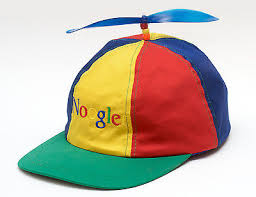
\includegraphics[width=\linewidth]{noogler.jpg}
\end{minipage}

\noindent\textcolor{primary}{\rule{\linewidth}{3pt}}
% \noindent\makebox[\linewidth]{\rule{\linewidth}{1pt}}
% ----------------------------------------------------------------------------------------
\color{DarkSlateGray}
\scalefont{1.1}


\section*{Motivation}
We need a tool to discover all shared library dependencies across modules in an Android device.
Although we have some tools existing, it's still far from sufficient.
These hidden dependencies undermine the foundation of Treble project.

\begin{multicols}{2}
  \section*{SourceDR}
  \subsection*{Overview}
  Basically, sourceDR is a tool to discover all shared library dependencies across modules in an Android device. The aim of this tool is to accelerate the process of labeling dependencies and save time for reviewers when the source code gets modified.
  \subsection*{Features}
      {\color{secondary}
        \begin{itemize}
        \item web-based UI
        \item embedded syntax highlighter(prism)
        \item jump to pattern line
        \item integrate with google code search to accelerate process
        \item temporary grep-like search
        \item similar entries suggestion
        \end{itemize}
      }
  \subsection*{Implementation}
    \subsubsection*{Programming Languages Used}
    {\color{secondary}
      \begin{itemize}
      \item Python
      \item Javascript(jQuery)
      \item Html/Css
      \end{itemize}
    }
    \subsubsection*{Tools and Frameworks}
    {\color{secondary}
      \begin{itemize}
      \item Flask backend
      \item Prism, a syntax highlighter
      \end{itemize}
    }
    \subsection*{User Interface}
    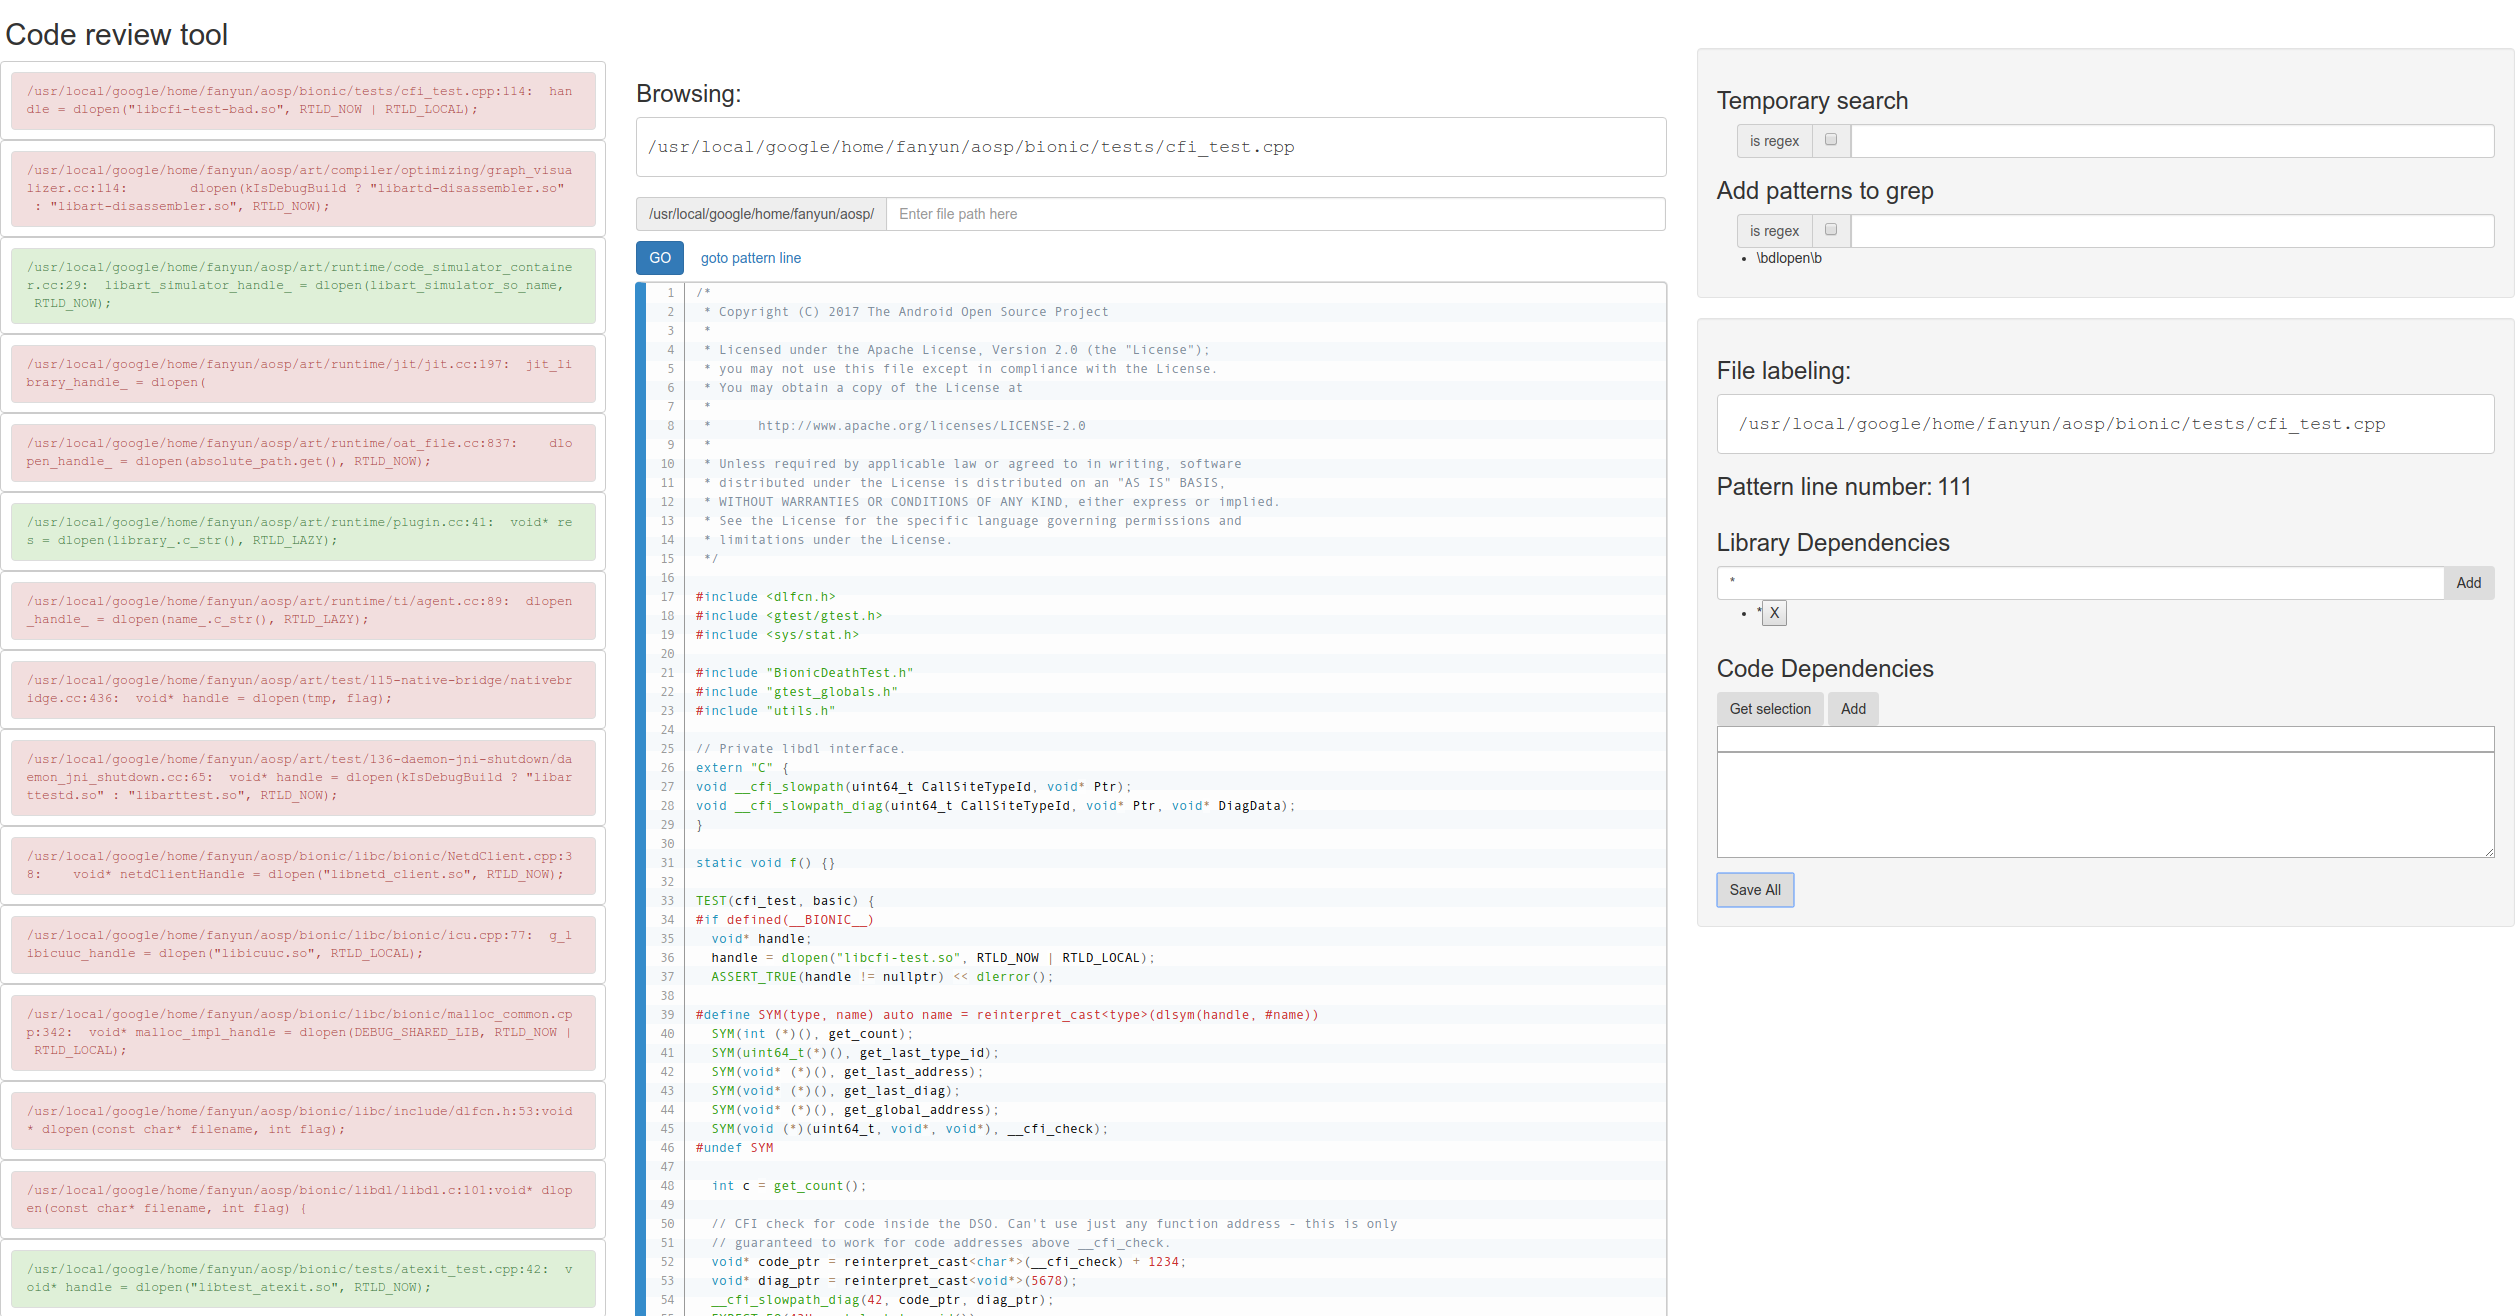
\includegraphics[width=\linewidth]{screenshot.png}

\columnbreak
  \section*{LoadLibAnalyzer}
  \subsection*{Overview}
  LoadLibAnalyzer is a tool that aims to find out all possile arguments of all invocations to System.loadLibrary(). After constructing a control flow graph from reading Dalvik bytecode, we perform a data flow analysis on the flow graph.
  \subsection*{Examples}
  \begin{lstlisting}
  public class Test {
    public static void main(String args[]) {
        String libName;
        if (args.length > 5) {
            libName = "liba";
        } else {
            libName = "libb";
        }
        System.loadLibrary(libName);
    }
  }
  \end{lstlisting}
  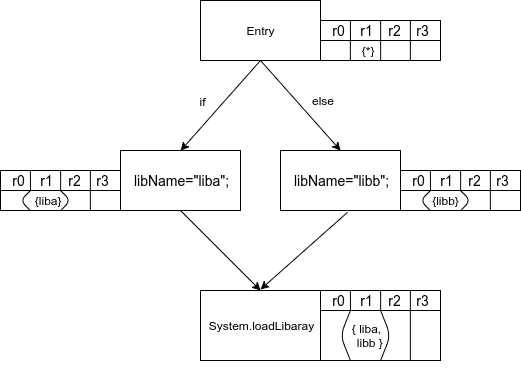
\includegraphics[width=\linewidth]{data_flow.png}

  \subsection*{Implementation}
    \subsubsection*{Programming Languages Used}
    {\color{secondary}
      \begin{itemize}
      \item Java
      \end{itemize}
    }
    \subsubsection*{Tools and Frameworks}
    {\color{secondary}
      \begin{itemize}
      \item Soot, a Java analysis and optimization framework
      \item Maven
      \end{itemize}
    }

% switch off pager numbering
\pagenumbering{gobble}
\end{multicols}
\end{document}
